\documentclass[conference]{IEEEtran}
\IEEEoverridecommandlockouts

% Packages
\usepackage{cite}
\usepackage{amsmath,amssymb,amsfonts}
\usepackage{algorithmic}
\usepackage{graphicx}
\usepackage{textcomp}
\usepackage{xcolor}
\usepackage{booktabs}
\usepackage{multirow}
\usepackage{url}
\usepackage{hyperref}
\usepackage{siunitx}
\usepackage{pgfplots}
\pgfplotsset{compat=1.18}
\usepgfplotslibrary{groupplots}
\usepackage{tikz}
\usepackage{balance}
\usepackage{subcaption}

\def\BibTeX{{\rm B\kern-.05em{\sc i\kern-.025em b}\kern-.08em
    T\kern-.1667em\lower.7ex\hbox{E}\kern-.125emX}}

% Color definitions for consistent styling
\definecolor{webglblue}{HTML}{2E86DE}
\definecolor{webgpured}{HTML}{E74C3C}
\definecolor{webgllight}{HTML}{74B9FF}
\definecolor{webgpulight}{HTML}{FC8D8D}

\begin{document}

\title{A Comparative Performance Analysis of WebGL~2.0 and WebGPU for Real-Time Browser-Based 3D Rendering and General-Purpose GPU Computing}

\author{
\IEEEauthorblockN{Vinay N}
\IEEEauthorblockA{
Department of Computer Science\\
\textit{Independent Research}\\
Email: \texttt{vinay@example.com}}
}

\maketitle

\begin{abstract}
The evolution of web-based graphics APIs has reached an inflection point with the emergence of WebGPU as a successor to the long-established WebGL standard. This paper presents a rigorous, automated benchmarking study comparing WebGL~2.0 and WebGPU across five carefully designed rendering and compute scenarios: baseline rendering overhead, instanced geometry scaling, particle system simulation, general-purpose GPU (GPGPU) matrix multiplication, and per-object state-change stress testing. All experiments were conducted using a custom-built, open-source benchmarking framework with Puppeteer-based automation, ensuring statistical repeatability through 10 independent runs per configuration at a fixed 1280$\times$720 resolution with V-Sync disabled. Our results reveal that WebGPU delivers superior frame throughput in geometry-intensive workloads, achieving up to 2.34$\times$ higher FPS than WebGL at 1{,}000 instanced cubes, while simultaneously reducing CPU-side overhead by 89.6\% in particle simulations at 200{,}000 particles. However, WebGPU exhibits substantially higher initialization latency---up to 17.3$\times$ for baseline scenarios---and demonstrates significantly degraded performance in state-change-heavy rendering patterns, dropping to as low as 5.94 FPS versus WebGL's 80.78 FPS at 10{,}000 objects. These findings provide empirically grounded guidance for developers evaluating migration from WebGL to WebGPU, identifying the workload characteristics under which each API excels.
\end{abstract}

\begin{IEEEkeywords}
WebGL, WebGPU, GPU computing, browser-based rendering, performance benchmarking, real-time graphics, compute shaders, GPGPU
\end{IEEEkeywords}

%----------------------------------------------------------------------
\section{Introduction}
\label{sec:introduction}

Browser-based 3D graphics have become a cornerstone of modern web applications, powering interactive visualizations, browser games, virtual reality experiences, data-driven dashboards, and scientific simulations~\cite{evans2014webgl, cabello2010threejs}. For over a decade, WebGL---first standardized by the Khronos Group in 2011 and later updated to WebGL~2.0 in 2017---has served as the dominant API for hardware-accelerated rendering in the browser~\cite{khronos2017webgl2}. Built atop OpenGL ES, WebGL provides a well-understood programming model with broad compatibility across desktop and mobile platforms.

However, WebGL's architecture inherits fundamental limitations from its OpenGL ES lineage. Its single-threaded, immediate-mode state machine model incurs significant CPU overhead for every draw call, texture binding, and uniform update~\cite{sellers2016vulkan}. As web applications demand increasingly complex scenes with thousands of independently rendered objects, WebGL's per-draw-call overhead becomes a critical bottleneck. Furthermore, WebGL lacks native support for general-purpose GPU computing (GPGPU), forcing developers to resort to workarounds such as rendering to floating-point textures, which adds programming complexity and reduces efficiency~\cite{cabello2010threejs}.

WebGPU, developed by the W3C GPU for the Web Community Group, represents a paradigm shift in browser-based graphics~\cite{w3c2024webgpu}. Inspired by modern, low-overhead native APIs---including Vulkan~\cite{sellers2016vulkan}, Direct3D~12~\cite{microsoft2015dx12}, and Metal~\cite{apple2014metal}---WebGPU introduces explicit resource management, pipeline state objects, command buffer recording, and first-class compute shader support. These architectural changes promise reduced driver overhead, improved multi-threading potential, and native GPGPU capabilities.

Despite the theoretical advantages of WebGPU, the question of practical, measurable performance differences under controlled conditions remains insufficiently studied. Existing comparisons are often anecdotal, rely on single benchmarks, or fail to account for statistical variance across runs~\cite{nickolls2010gpu}. This paper addresses this gap by presenting a comprehensive, automated benchmarking study that:

\begin{enumerate}
    \item Designs five distinct benchmark scenarios isolating different aspects of GPU and API performance (Section~\ref{sec:methodology}).
    \item Employs rigorous experimental methodology with automated browser-based test execution, 10 repeated runs per configuration, and statistical aggregation including standard deviation and 95th-percentile latency metrics (Section~\ref{sec:experimental}).
    \item Presents detailed quantitative results comparing mean FPS, frame time, CPU time, and initialization latency across both APIs (Section~\ref{sec:results}).
    \item Analyzes the conditions under which each API excels or underperforms, providing actionable guidance for web developers and researchers (Section~\ref{sec:discussion}).
\end{enumerate}

%----------------------------------------------------------------------
\section{Background and Related Work}
\label{sec:background}

\subsection{WebGL 2.0}

WebGL~2.0 is a JavaScript API that exposes OpenGL ES~3.0 functionality within the browser~\cite{khronos2017webgl2}. It operates through an \texttt{HTMLCanvasElement}, providing a rendering context that supports vertex and fragment shaders written in GLSL ES~3.00, vertex array objects (VAOs), instanced drawing, multiple render targets, and floating-point textures. WebGL~2.0 follows a stateful, immediate-mode programming model: developers set global state (active program, bound textures, blend mode) and issue draw calls that execute against this state. While this model is conceptually straightforward, it requires the browser and driver to perform extensive validation on each state change and draw call, incurring CPU-side overhead that becomes significant at high draw-call counts~\cite{sellers2016vulkan}.

\subsection{WebGPU}

WebGPU is a new web standard~\cite{w3c2024webgpu} designed to provide modern, low-overhead access to GPU hardware. Unlike WebGL, WebGPU uses an explicit programming model where resources (buffers, textures, samplers) are created independently and composed into immutable \textit{bind groups}. Rendering and compute configurations are encapsulated in pre-validated \textit{pipeline state objects}, eliminating per-draw-call validation overhead at runtime. Commands are recorded into \textit{command buffers} that are submitted to the GPU queue as atomic units, enabling efficient batching and potential multi-threaded command encoding~\cite{beaufort2023webgpu}.

A distinguishing feature of WebGPU is native compute shader support through the WebGPU Shading Language (WGSL)~\cite{w3c2024wgsl}. Compute shaders enable direct GPU-parallel algorithms without the overhead of configuring a rendering pipeline---a capability that WebGL can only approximate through GPGPU techniques involving render-to-texture passes.

\subsection{Related Benchmarking Studies}

Prior work on GPU API benchmarking has primarily focused on native APIs. Kessenich et al.~\cite{kessenich2018opengl} provided foundational comparisons between OpenGL and Vulkan draw-call overhead. Sellers~\cite{sellers2016vulkan} demonstrated Vulkan's advantages for multi-threaded rendering. In the web context, Evans~\cite{evans2014webgl} characterized WebGL performance for scientific visualization. However, systematic comparisons between WebGL and WebGPU using controlled browser-automated benchmarks with statistical rigor remain scarce. Beaufort~\cite{beaufort2023webgpu} provided an overview of WebGPU capabilities but did not present quantitative performance data. Our work fills this gap with a multi-scenario, multi-metric benchmarking framework.

%----------------------------------------------------------------------
\section{Methodology}
\label{sec:methodology}

\subsection{Benchmarking Framework Architecture}

We developed a custom open-source benchmarking framework consisting of the following components:

\begin{itemize}
    \item \textbf{Scenario Engine}: A base \texttt{Scenario} class providing standardized initialization, render-loop management via \texttt{requestAnimationFrame}, and harness integration. Each benchmark scenario extends this class with API-specific (\texttt{WebGL} or \texttt{WebGPU}) implementations.
    \item \textbf{Metrics Harness}: A \texttt{BenchmarkHarness} class that manages timing with a 1-second warmup phase followed by a 3-second active measurement window. The harness records per-frame timestamps using \texttt{performance.now()}, measures CPU time via \texttt{performance.mark/measure}, and optionally captures GPU timestamps using WebGPU's \texttt{timestamp-query} feature.
    \item \textbf{Automation Runner}: A Node.js script using Puppeteer~\cite{puppeteer2024} to launch headless Chromium with \texttt{--enable-unsafe-webgpu} and \texttt{--disable-frame-rate-limit} flags, iterate over the full test matrix, and collect results programmatically.
    \item \textbf{Shared Math Library}: A minimal, dependency-free matrix library providing \texttt{mat4} operations (perspective projection, translation, rotation) used identically by both API implementations, ensuring computational parity.
\end{itemize}

\subsection{Benchmark Scenarios}

Five benchmark scenarios were designed to isolate distinct performance characteristics:

\subsubsection{Scenario A --- Baseline Rendering}
A single textured, lit, rotating cube is rendered to measure the minimum per-frame overhead of each API, including context setup, shader dispatch, and frame submission. This scenario establishes the performance floor.

\subsubsection{Scenario B --- Geometry Scaling (Instanced Rendering)}
Between 100 and 10{,}000 cubes are rendered using hardware-instanced rendering (\texttt{drawElementsInstanced} in WebGL; \texttt{renderPass.drawIndexed} with instance count in WebGPU). Each frame updates per-instance transformation matrices (translation + rotation) and uploads them to GPU buffers. This scenario measures how each API handles increasing vertex and instance throughput.

\subsubsection{Scenario C --- Particle System (Compute vs. CPU Physics)}
A particle simulation with counts ranging from 10{,}000 to 200{,}000 particles tests data-parallel computation. In WebGPU, particle positions and velocities are updated entirely on the GPU using a compute shader dispatched with 64-thread workgroups. In WebGL, the same physics simulation runs on the CPU via \texttt{Float32Array} manipulation, with updated positions uploaded to the GPU each frame via \texttt{bufferSubData}. This scenario directly isolates the compute advantage of WebGPU.

\subsubsection{Scenario D --- GPGPU Matrix Multiplication}
Square matrix multiplication (dimensions derived from the \texttt{count} parameter, up to 1024$\times$1024) is performed using native compute shaders in WebGPU (\texttt{@compute @workgroup\_size(8,8)} dispatched over the matrix dimensions) and GPGPU techniques in WebGL (fragment shader reads from two \texttt{R32F} textures, writes to a framebuffer-attached texture). This scenario compares computational throughput for a purely compute-bound workload.

\subsubsection{Scenario E --- State-Change Stress Test}
Between 500 and 10{,}000 objects are rendered without instancing, requiring per-object uniform updates (model-view matrix and color) and individual draw calls. In WebGL, this means per-object \texttt{uniformMatrix4fv} and \texttt{drawElements} calls. In WebGPU, each object requires a separate bind group and draw call within the render pass. This scenario measures the overhead of API state changes at scale.

\subsection{Metrics Collected}

For each test configuration (API $\times$ Scenario $\times$ Count), the following metrics are collected over 10 independent runs:

\begin{itemize}
    \item \textbf{Mean FPS}: Average frames per second during the 3-second measurement window.
    \item \textbf{FPS Standard Deviation ($\sigma_{\text{FPS}}$)}: Inter-run variability.
    \item \textbf{Mean Frame Time}: Average time per frame in milliseconds.
    \item \textbf{95th Percentile Frame Time (P95)}: Tail latency metric capturing worst-case frame times.
    \item \textbf{Mean CPU Time}: Average JavaScript/CPU execution time per frame.
    \item \textbf{Mean Initialization Time}: Time from context creation to first frame.
\end{itemize}

%----------------------------------------------------------------------
\section{Experimental Setup}
\label{sec:experimental}

All benchmarks were executed on a system running Windows~10 (64-bit), using a Puppeteer-controlled headless Chromium browser (version~145.0.0.0). The rendering resolution was fixed at 1280$\times$720 pixels. V-Sync was disabled via \texttt{--disable-gpu-vsync} and \texttt{--disable-frame-rate-limit} flags to enable uncapped frame rate measurement.

Each test configuration was executed 10 times (\texttt{NUM\_RUNS = 10}) with a per-run timeout of 120 seconds. The benchmark harness enforced a 1-second warmup period (discarded frames) followed by a 3-second active recording period. Results were aggregated into mean, standard deviation, and P95 statistics across the 10 runs.

The test matrix comprised 2 APIs $\times$ 18 unique (Scenario, Count) configurations, yielding 36 distinct test cases, each repeated 10 times for a total of 360 benchmark executions. Results were exported as both JSON and CSV for analysis.

%----------------------------------------------------------------------
\section{Results}
\label{sec:results}

\subsection{Scenario A: Baseline Rendering}

Table~\ref{tab:scenario_a} and Fig.~\ref{fig:scenario_a_bar} show the baseline performance for rendering a single rotating cube.

\begin{table}[htbp]
\caption{Scenario A --- Baseline Rendering (Single Cube)}
\label{tab:scenario_a}
\centering
\begin{tabular}{@{}lcc@{}}
\toprule
\textbf{Metric} & \textbf{WebGL 2.0} & \textbf{WebGPU} \\
\midrule
Mean FPS & 1098.40 & 678.82 \\
Std FPS ($\sigma$) & 27.95 & 51.51 \\
Mean Frame Time (ms) & 0.91 & 1.48 \\
P95 Frame Time (ms) & 2.02 & 2.54 \\
Mean CPU Time (ms) & 0.12 & 0.37 \\
Mean Init Time (ms) & 6.07 & 104.78 \\
\bottomrule
\end{tabular}
\end{table}

\begin{figure}[htbp]
\centering
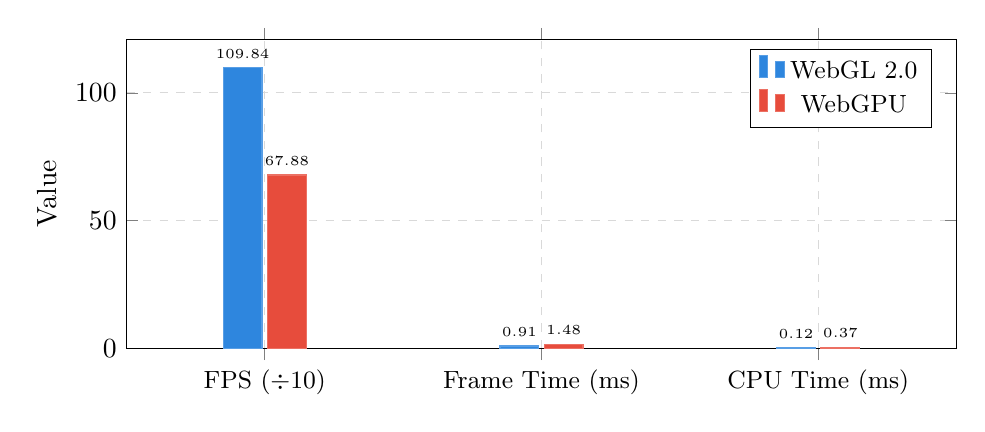
\begin{tikzpicture}
\begin{axis}[
    ybar,
    width=\columnwidth,
    height=5.5cm,
    bar width=14pt,
    ylabel={Value},
    symbolic x coords={FPS ($\div$10), Frame Time (ms), CPU Time (ms)},
    xtick=data,
    x tick label style={font=\small},
    ymin=0,
    legend pos=north east,
    legend style={font=\small},
    grid=major,
    grid style={dashed, gray!30},
    nodes near coords,
    nodes near coords style={font=\tiny, above},
    every node near coord/.append style={rotate=0},
    enlarge x limits=0.25
]
\addplot[fill=webglblue, draw=webglblue!80] coordinates {
    (FPS ($\div$10), 109.84)
    (Frame Time (ms), 0.91)
    (CPU Time (ms), 0.12)
};
\addplot[fill=webgpured, draw=webgpured!80] coordinates {
    (FPS ($\div$10), 67.88)
    (Frame Time (ms), 1.48)
    (CPU Time (ms), 0.37)
};
\legend{WebGL 2.0, WebGPU}
\end{axis}
\end{tikzpicture}
\caption{Scenario A: Baseline performance comparison. FPS values are scaled by $\div$10 for readability. WebGL achieves 1.62$\times$ higher FPS with 3.1$\times$ lower CPU overhead.}
\label{fig:scenario_a_bar}
\end{figure}

WebGL achieves 1.62$\times$ higher FPS than WebGPU in this minimal workload. The result reflects WebGPU's higher per-frame API overhead for command buffer creation and submission. WebGPU's initialization time is 17.3$\times$ larger due to adapter negotiation, device creation, and pipeline compilation.

\subsection{Scenario B: Instanced Geometry Scaling}

Fig.~\ref{fig:scenario_b_fps} and Table~\ref{tab:scenario_b} present the FPS scaling results, while Fig.~\ref{fig:scenario_b_frametime} illustrates the corresponding frame time and CPU time decomposition.

\begin{table}[htbp]
\caption{Scenario B --- Instanced Geometry Scaling (Complete Metrics)}
\label{tab:scenario_b}
\centering
\small
\begin{tabular}{@{}rrrrrrr@{}}
\toprule
 & \multicolumn{2}{c}{\textbf{Mean FPS}} & \multicolumn{2}{c}{\textbf{CPU Time (ms)}} & \multicolumn{2}{c}{\textbf{P95 (ms)}} \\
\cmidrule(lr){2-3} \cmidrule(lr){4-5} \cmidrule(lr){6-7}
\textbf{N} & \textbf{GL} & \textbf{GPU} & \textbf{GL} & \textbf{GPU} & \textbf{GL} & \textbf{GPU} \\
\midrule
100 & 816.84 & 640.63 & 0.36 & 0.45 & 2.35 & 2.62 \\
500 & 313.07 & 506.49 & 2.59 & 0.69 & 22.03 & 3.53 \\
1K & 162.69 & 380.71 & 5.39 & 1.21 & 53.88 & 4.09 \\
5K & 106.74 & 225.59 & 8.50 & 2.95 & 44.80 & 6.27 \\
10K & 110.41 & 182.53 & 8.25 & 4.52 & 33.10 & 7.11 \\
\bottomrule
\end{tabular}
\end{table}

\begin{figure}[htbp]
\centering
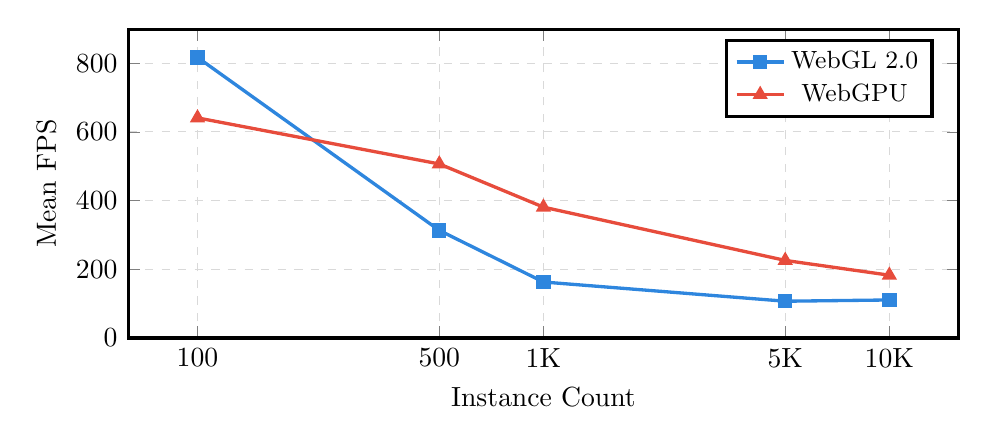
\begin{tikzpicture}
\begin{axis}[
    width=\columnwidth,
    height=5.5cm,
    xlabel={Instance Count},
    ylabel={Mean FPS},
    legend pos=north east,
    legend style={font=\small},
    grid=major,
    grid style={dashed, gray!30},
    xmode=log,
    log basis x={10},
    ymin=0,
    xtick={100,500,1000,5000,10000},
    xticklabels={100,500,1K,5K,10K},
    mark size=2pt,
    line width=1.2pt
]
\addplot[color=webglblue, mark=square*, mark options={fill=webglblue}] coordinates {
    (100, 816.84)
    (500, 313.07)
    (1000, 162.69)
    (5000, 106.74)
    (10000, 110.41)
};
\addlegendentry{WebGL 2.0}

\addplot[color=webgpured, mark=triangle*, mark options={fill=webgpured}] coordinates {
    (100, 640.63)
    (500, 506.49)
    (1000, 380.71)
    (5000, 225.59)
    (10000, 182.53)
};
\addlegendentry{WebGPU}
\end{axis}
\end{tikzpicture}
\caption{Scenario B: Mean FPS vs.\ instance count. WebGPU overtakes WebGL at $\sim$200 instances and maintains a 1.6--2.3$\times$ advantage up to 10{,}000 instances.}
\label{fig:scenario_b_fps}
\end{figure}

\begin{figure}[htbp]
\centering
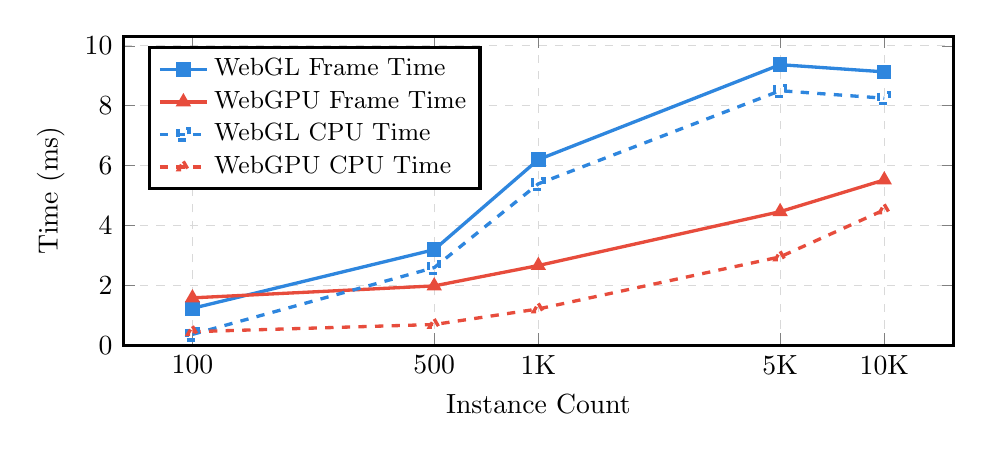
\begin{tikzpicture}
\begin{axis}[
    width=\columnwidth,
    height=5.5cm,
    xlabel={Instance Count},
    ylabel={Time (ms)},
    legend pos=north west,
    legend style={font=\small, cells={anchor=west}},
    grid=major,
    grid style={dashed, gray!30},
    xmode=log,
    log basis x={10},
    ymin=0,
    xtick={100,500,1000,5000,10000},
    xticklabels={100,500,1K,5K,10K},
    mark size=2pt,
    line width=1.2pt
]
\addplot[color=webglblue, mark=square*, mark options={fill=webglblue}] coordinates {
    (100, 1.23) (500, 3.19) (1000, 6.20) (5000, 9.37) (10000, 9.13)
};
\addlegendentry{WebGL Frame Time}

\addplot[color=webgpured, mark=triangle*, mark options={fill=webgpured}] coordinates {
    (100, 1.58) (500, 1.98) (1000, 2.66) (5000, 4.46) (10000, 5.52)
};
\addlegendentry{WebGPU Frame Time}

\addplot[color=webglblue, mark=square, dashed, mark options={fill=webgllight}] coordinates {
    (100, 0.36) (500, 2.59) (1000, 5.39) (5000, 8.50) (10000, 8.25)
};
\addlegendentry{WebGL CPU Time}

\addplot[color=webgpured, mark=triangle, dashed, mark options={fill=webgpulight}] coordinates {
    (100, 0.45) (500, 0.69) (1000, 1.21) (5000, 2.95) (10000, 4.52)
};
\addlegendentry{WebGPU CPU Time}
\end{axis}
\end{tikzpicture}
\caption{Scenario B: Frame time and CPU time decomposition. WebGL's CPU time dominates its frame time (ratio $>$0.9), indicating CPU-boundedness. WebGPU's CPU share remains below 0.82 at all counts.}
\label{fig:scenario_b_frametime}
\end{figure}

WebGPU surpasses WebGL at approximately 200 instances and maintains a 1.6--2.3$\times$ FPS advantage through 10{,}000 instances. The CPU time decomposition in Fig.~\ref{fig:scenario_b_frametime} reveals the underlying mechanism: WebGL's CPU time (8.50~ms at 5K instances) accounts for over 90\% of its frame time (9.37~ms), confirming that WebGL is CPU-bound in this scenario. WebGPU's CPU time (2.95~ms) represents only 66\% of its frame time (4.46~ms), indicating better utilization of GPU parallelism.

\subsection{Scenario B: Tail Latency Analysis}

Fig.~\ref{fig:scenario_b_p95} shows the 95th-percentile frame time, a critical metric for interactive applications where occasional frame spikes cause perceptible stutter.

\begin{figure}[htbp]
\centering
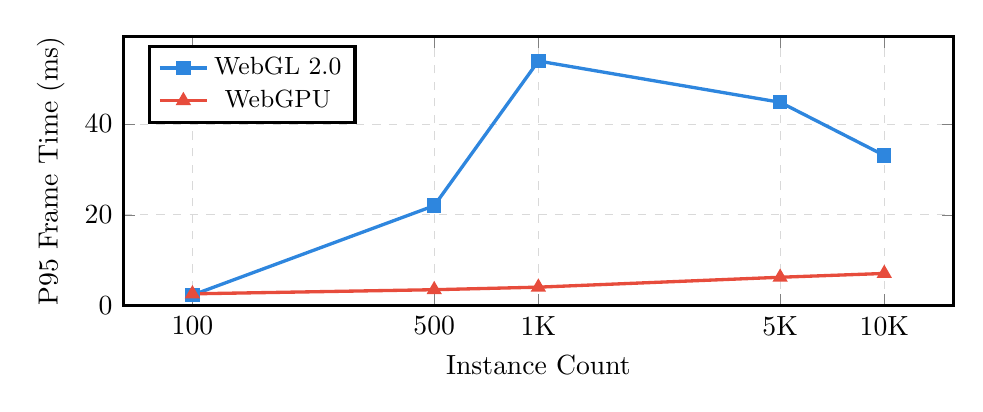
\begin{tikzpicture}
\begin{axis}[
    width=\columnwidth,
    height=5cm,
    xlabel={Instance Count},
    ylabel={P95 Frame Time (ms)},
    legend pos=north west,
    legend style={font=\small},
    grid=major,
    grid style={dashed, gray!30},
    xmode=log,
    log basis x={10},
    ymin=0,
    xtick={100,500,1000,5000,10000},
    xticklabels={100,500,1K,5K,10K},
    mark size=2pt,
    line width=1.2pt
]
\addplot[color=webglblue, mark=square*, mark options={fill=webglblue}] coordinates {
    (100, 2.35) (500, 22.03) (1000, 53.88) (5000, 44.80) (10000, 33.10)
};
\addlegendentry{WebGL 2.0}

\addplot[color=webgpured, mark=triangle*, mark options={fill=webgpured}] coordinates {
    (100, 2.62) (500, 3.53) (1000, 4.09) (5000, 6.27) (10000, 7.11)
};
\addlegendentry{WebGPU}
\end{axis}
\end{tikzpicture}
\caption{Scenario B: 95th-percentile frame time. WebGL exhibits severe tail latency spikes (53.88~ms at 1K instances), while WebGPU maintains smooth, predictable frame pacing ($<$8~ms at all counts).}
\label{fig:scenario_b_p95}
\end{figure}

WebGL's P95 frame time spikes to 53.88~ms at 1{,}000 instances---a 8.7$\times$ ratio over its mean frame time (6.20~ms)---indicating severe frame time variance likely caused by driver-side batching or garbage collection stalls. WebGPU's P95 remains below 7.11~ms across all counts, with a maximum P95-to-mean ratio of only 1.54$\times$, indicating significantly more consistent frame delivery.

\subsection{Scenario C: Particle System}

Table~\ref{tab:scenario_c} and Fig.~\ref{fig:scenario_c} compare particle system performance, with separate panels for FPS throughput and CPU time.

\begin{table}[htbp]
\caption{Scenario C --- Particle System (Complete Metrics)}
\label{tab:scenario_c}
\centering
\small
\begin{tabular}{@{}rrrrrr@{}}
\toprule
 & \multicolumn{2}{c}{\textbf{Mean FPS}} & \multicolumn{2}{c}{\textbf{CPU Time (ms)}} & \textbf{CPU} \\
\cmidrule(lr){2-3} \cmidrule(lr){4-5}
\textbf{Particles} & \textbf{GL} & \textbf{GPU} & \textbf{GL} & \textbf{GPU} & \textbf{Savings} \\
\midrule
10K & 652.28 & 645.69 & 0.47 & 0.34 & 27.7\% \\
50K & 415.09 & 369.63 & 1.51 & 0.43 & 71.5\% \\
100K & 325.30 & 241.88 & 2.43 & 0.53 & 78.2\% \\
200K & 208.46 & 155.32 & 4.41 & 0.46 & 89.6\% \\
\bottomrule
\end{tabular}
\end{table}

\begin{figure}[htbp]
\centering
\begin{tikzpicture}
\begin{groupplot}[
    group style={
        group size=1 by 2,
        vertical sep=1.2cm,
        xlabels at=edge bottom,
    },
    width=\columnwidth,
    height=4cm,
    xmode=log,
    log basis x={10},
    xtick={10000,50000,100000,200000},
    xticklabels={10K,50K,100K,200K},
    grid=major,
    grid style={dashed, gray!30},
    mark size=2pt,
    line width=1.2pt,
    legend style={font=\small}
]

% Top panel: FPS
\nextgroupplot[
    ylabel={Mean FPS},
    ymin=0, ymax=700,
    legend pos=north east,
]
\addplot[color=webglblue, mark=square*, mark options={fill=webglblue}] coordinates {
    (10000, 652.28) (50000, 415.09) (100000, 325.30) (200000, 208.46)
};
\addlegendentry{WebGL 2.0}
\addplot[color=webgpured, mark=triangle*, mark options={fill=webgpured}] coordinates {
    (10000, 645.69) (50000, 369.63) (100000, 241.88) (200000, 155.32)
};
\addlegendentry{WebGPU}

% Bottom panel: CPU Time
\nextgroupplot[
    xlabel={Particle Count},
    ylabel={CPU Time (ms)},
    ymin=0, ymax=5,
    legend pos=north west,
]
\addplot[color=webglblue, mark=square*, mark options={fill=webglblue}] coordinates {
    (10000, 0.47) (50000, 1.51) (100000, 2.43) (200000, 4.41)
};
\addlegendentry{WebGL (CPU Physics)}
\addplot[color=webgpured, mark=triangle*, mark options={fill=webgpured}] coordinates {
    (10000, 0.34) (50000, 0.43) (100000, 0.53) (200000, 0.46)
};
\addlegendentry{WebGPU (Compute Shader)}

\end{groupplot}
\end{tikzpicture}
\caption{Scenario C: \textit{Top}: Mean FPS. WebGL maintains higher raw FPS due to simpler frame submission. \textit{Bottom}: CPU time. WebGL scales linearly ($O(n)$) while WebGPU remains constant ($<$0.6~ms), demonstrating the compute shader advantage.}
\label{fig:scenario_c}
\end{figure}

While WebGL achieves higher raw FPS in this scenario (due to simpler overall frame submission overhead), the CPU time data reveals the fundamental architectural difference. WebGL's CPU time scales linearly from 0.47~ms (10K particles) to 4.41~ms (200K particles) as the CPU must iterate over every particle for the physics update. WebGPU's CPU time remains nearly constant at $\sim$0.46~ms regardless of particle count, as all physics computation occurs on the GPU via compute shaders. At 200{,}000 particles, WebGPU reduces CPU overhead by 89.6\%, freeing the main JavaScript thread for application logic.

\subsection{Scenario D: GPGPU Matrix Multiplication}

Table~\ref{tab:scenario_d} and Fig.~\ref{fig:scenario_d} show compute performance and the dramatic initialization overhead contrast.

\begin{table}[htbp]
\caption{Scenario D --- Matrix Multiplication (Complete Metrics)}
\label{tab:scenario_d}
\centering
\small
\begin{tabular}{@{}rcccccc@{}}
\toprule
 & \multicolumn{2}{c}{\textbf{Mean FPS}} & \multicolumn{2}{c}{\textbf{Frame Time}} & \multicolumn{2}{c}{\textbf{Init (ms)}} \\
\cmidrule(lr){2-3} \cmidrule(lr){4-5} \cmidrule(lr){6-7}
\textbf{Size} & \textbf{GL} & \textbf{GPU} & \textbf{GL} & \textbf{GPU} & \textbf{GL} & \textbf{GPU} \\
\midrule
100 & 907.52 & 819.95 & 1.10 & 1.22 & 7.38 & 374.20 \\
256 & 910.35 & 823.68 & 1.10 & 1.22 & 6.07 & 137.57 \\
512 & 903.81 & 849.66 & 1.11 & 1.18 & 5.64 & 194.80 \\
1024 & 910.36 & 804.36 & 1.10 & 1.25 & 4.83 & 180.31 \\
\bottomrule
\end{tabular}
\end{table}

\begin{figure}[htbp]
\centering
\begin{tikzpicture}
\begin{groupplot}[
    group style={
        group size=1 by 2,
        vertical sep=1.2cm,
        xlabels at=edge bottom,
    },
    width=\columnwidth,
    height=4cm,
    grid=major,
    grid style={dashed, gray!30},
    mark size=2pt,
    line width=1.2pt,
    legend style={font=\small},
    xtick={100,256,512,1024},
    xticklabels={100,256,512,1024}
]

% Top panel: FPS
\nextgroupplot[
    ylabel={Mean FPS},
    ymin=700, ymax=950,
    legend pos=south west,
]
\addplot[color=webglblue, mark=square*, mark options={fill=webglblue}] coordinates {
    (100, 907.52) (256, 910.35) (512, 903.81) (1024, 910.36)
};
\addlegendentry{WebGL (GPGPU)}
\addplot[color=webgpured, mark=triangle*, mark options={fill=webgpured}] coordinates {
    (100, 819.95) (256, 823.68) (512, 849.66) (1024, 804.36)
};
\addlegendentry{WebGPU (Compute)}

% Bottom panel: Init time
\nextgroupplot[
    xlabel={Matrix Dimension ($N \times N$)},
    ylabel={Init Time (ms)},
    ymin=0,
    legend pos=north east,
    ymode=log,
    log basis y={10},
]
\addplot[color=webglblue, mark=square*, mark options={fill=webglblue}] coordinates {
    (100, 7.38) (256, 6.07) (512, 5.64) (1024, 4.83)
};
\addlegendentry{WebGL 2.0}
\addplot[color=webgpured, mark=triangle*, mark options={fill=webgpured}] coordinates {
    (100, 374.20) (256, 137.57) (512, 194.80) (1024, 180.31)
};
\addlegendentry{WebGPU}

\end{groupplot}
\end{tikzpicture}
\caption{Scenario D: \textit{Top}: Steady-state FPS is comparable ($\sim$6--11\% WebGL advantage), confirming GPU-compute-bound behavior. \textit{Bottom}: Initialization time (log scale) shows 22--51$\times$ overhead for WebGPU pipeline creation.}
\label{fig:scenario_d}
\end{figure}

Both APIs achieve high FPS across all matrix sizes, with WebGL maintaining a slight edge (6--11\% higher FPS). This reflects the fact that both approaches fully offload computation to the GPU: WebGL through render-to-texture GPGPU, WebGPU through native compute shaders. The nearly identical FPS across matrix sizes suggests that the workload is GPU-compute-bound rather than API-overhead-bound. However, WebGPU's initialization overhead is 22--51$\times$ higher, primarily due to compute pipeline creation and shader module compilation.

\subsection{Scenario E: State-Change Stress Test}

Table~\ref{tab:scenario_e} and Fig.~\ref{fig:scenario_e} reveal the most dramatic performance divergence. Fig.~\ref{fig:scenario_e_frametime} presents the frame time decomposition with P95 overlay.

\begin{table}[htbp]
\caption{Scenario E --- State-Change Stress Test (Complete Metrics)}
\label{tab:scenario_e}
\centering
\small
\begin{tabular}{@{}rrrrrrl@{}}
\toprule
 & \multicolumn{2}{c}{\textbf{Mean FPS}} & \multicolumn{2}{c}{\textbf{$\sigma_{\text{FPS}}$}} & \\
\cmidrule(lr){2-3} \cmidrule(lr){4-5}
\textbf{N} & \textbf{GL} & \textbf{GPU} & \textbf{GL} & \textbf{GPU} & \textbf{Ratio} \\
\midrule
500 & 237.80 & 159.66 & 7.22 & 83.68 & 0.67$\times$ \\
2K & 113.87 & 38.92 & 2.04 & 30.48 & 0.34$\times$ \\
5K & 87.36 & 15.35 & 0.88 & 2.55 & 0.18$\times$ \\
10K & 80.78 & 5.94 & 1.51 & 0.27 & 0.07$\times$ \\
\bottomrule
\end{tabular}
\end{table}

\begin{figure}[htbp]
\centering
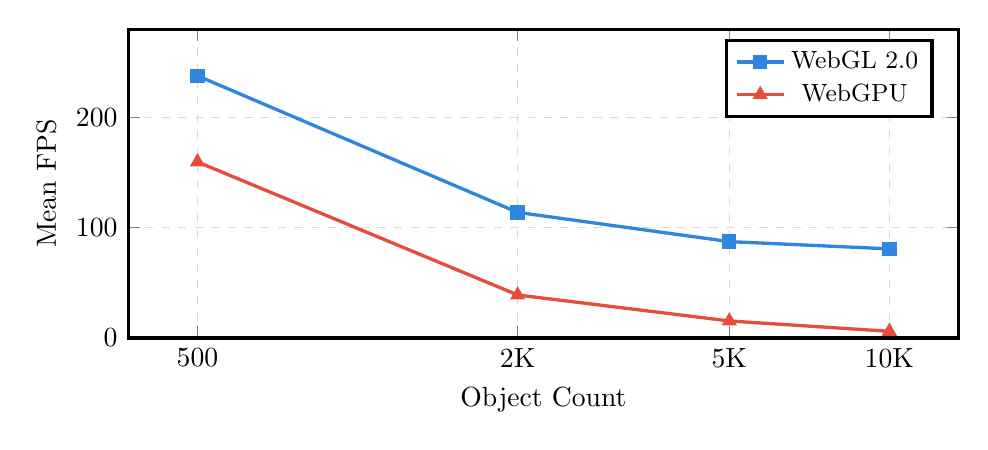
\begin{tikzpicture}
\begin{axis}[
    width=\columnwidth,
    height=5.5cm,
    xlabel={Object Count},
    ylabel={Mean FPS},
    legend pos=north east,
    legend style={font=\small},
    grid=major,
    grid style={dashed, gray!30},
    xmode=log,
    log basis x={10},
    ymin=0, ymax=280,
    xtick={500,2000,5000,10000},
    xticklabels={500,2K,5K,10K},
    mark size=2pt,
    line width=1.2pt
]
\addplot[color=webglblue, mark=square*, mark options={fill=webglblue}] coordinates {
    (500, 237.80) (2000, 113.87) (5000, 87.36) (10000, 80.78)
};
\addlegendentry{WebGL 2.0}

\addplot[color=webgpured, mark=triangle*, mark options={fill=webgpured}] coordinates {
    (500, 159.66) (2000, 38.92) (5000, 15.35) (10000, 5.94)
};
\addlegendentry{WebGPU}
\end{axis}
\end{tikzpicture}
\caption{Scenario E: Mean FPS under per-object state changes. WebGPU degrades exponentially, falling to 5.94 FPS at 10{,}000 objects---a 13.6$\times$ gap versus WebGL.}
\label{fig:scenario_e}
\end{figure}

\begin{figure}[htbp]
\centering
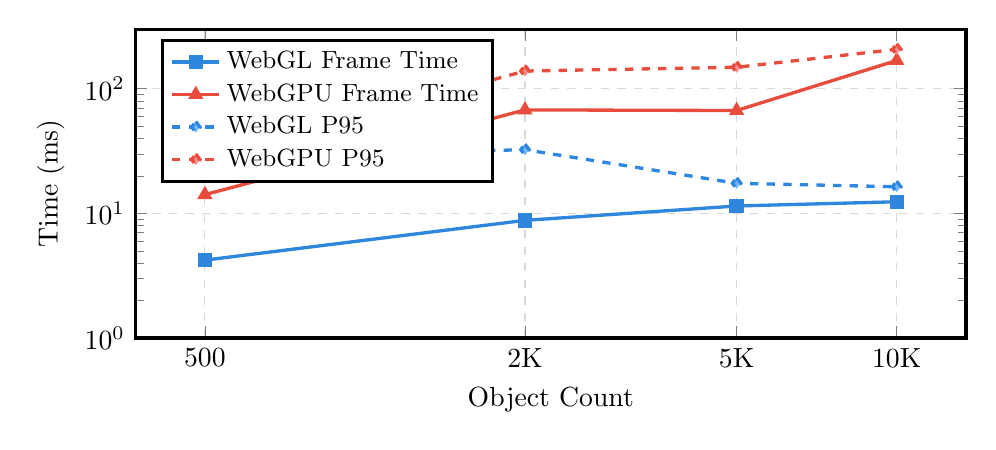
\begin{tikzpicture}
\begin{axis}[
    width=\columnwidth,
    height=5.5cm,
    xlabel={Object Count},
    ylabel={Time (ms)},
    legend pos=north west,
    legend style={font=\small, cells={anchor=west}},
    grid=major,
    grid style={dashed, gray!30},
    xmode=log,
    log basis x={10},
    ymode=log,
    log basis y={10},
    xtick={500,2000,5000,10000},
    xticklabels={500,2K,5K,10K},
    mark size=2pt,
    line width=1.2pt,
    ymin=1, ymax=300
]
\addplot[color=webglblue, mark=square*, mark options={fill=webglblue}] coordinates {
    (500, 4.21) (2000, 8.78) (5000, 11.45) (10000, 12.38)
};
\addlegendentry{WebGL Frame Time}

\addplot[color=webgpured, mark=triangle*, mark options={fill=webgpured}] coordinates {
    (500, 14.13) (2000, 67.65) (5000, 66.89) (10000, 168.65)
};
\addlegendentry{WebGPU Frame Time}

\addplot[color=webglblue, mark=diamond*, dashed, mark options={fill=webgllight}] coordinates {
    (500, 28.25) (2000, 32.41) (5000, 17.42) (10000, 16.34)
};
\addlegendentry{WebGL P95}

\addplot[color=webgpured, mark=diamond*, dashed, mark options={fill=webgpulight}] coordinates {
    (500, 27.82) (2000, 138.77) (5000, 148.83) (10000, 207.31)
};
\addlegendentry{WebGPU P95}
\end{axis}
\end{tikzpicture}
\caption{Scenario E: Frame time and P95 tail latency (log--log scale). WebGPU's P95 reaches 207.31~ms at 10K objects, confirming severe stutter. WebGL maintains sub-33~ms P95 across all counts.}
\label{fig:scenario_e_frametime}
\end{figure}

WebGPU exhibits severe performance degradation under high state-change workloads. At 10{,}000 objects, WebGPU achieves only 5.94~FPS with a mean frame time of 168.65~ms, compared to WebGL's 80.78~FPS and 12.38~ms frame time---a 13.6$\times$ performance gap. WebGPU's P95 frame time reaches 207.31~ms, far exceeding the 16.67~ms threshold for 60 FPS rendering. The high standard deviation in WebGPU's results ($\sigma_{\text{FPS}} = 83.68$ at 500 objects) also indicates significant frame-time instability across runs.

\subsection{Cross-Scenario Initialization Time Comparison}

Fig.~\ref{fig:init_time} and Table~\ref{tab:init_time} provide a comprehensive view of initialization overhead across all scenarios.

\begin{table}[htbp]
\caption{Mean Initialization Time (ms) Across Scenarios}
\label{tab:init_time}
\centering
\begin{tabular}{@{}lrrr@{}}
\toprule
\textbf{Scenario (Config)} & \textbf{WebGL} & \textbf{WebGPU} & \textbf{Ratio} \\
\midrule
A (Baseline) & 6.07 & 104.78 & 17.3$\times$ \\
B (1{,}000 inst.) & 8.86 & 303.02 & 34.2$\times$ \\
C (100K part.) & 12.62 & 149.12 & 11.8$\times$ \\
D (512 matmul) & 5.64 & 194.80 & 34.5$\times$ \\
E (5{,}000 obj.) & 6.72 & 1{,}439.14 & 214.2$\times$ \\
E (10{,}000 obj.) & 8.48 & 3{,}250.75 & 383.3$\times$ \\
\bottomrule
\end{tabular}
\end{table}

\begin{figure}[htbp]
\centering
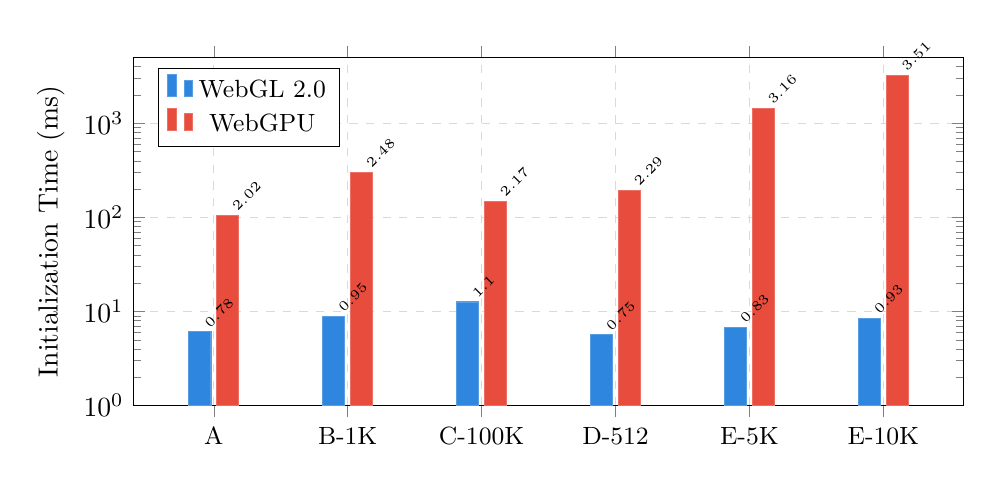
\begin{tikzpicture}
\begin{axis}[
    ybar,
    width=\columnwidth,
    height=6cm,
    bar width=8pt,
    ylabel={Initialization Time (ms)},
    ymode=log,
    log basis y={10},
    symbolic x coords={A, B-1K, C-100K, D-512, E-5K, E-10K},
    xtick=data,
    x tick label style={font=\small},
    ymin=1, ymax=5000,
    legend pos=north west,
    legend style={font=\small},
    grid=major,
    grid style={dashed, gray!30},
    enlarge x limits=0.12,
    nodes near coords,
    nodes near coords style={font=\tiny, rotate=45, anchor=west},
]
\addplot[fill=webglblue, draw=webglblue!80] coordinates {
    (A, 6.07)
    (B-1K, 8.86)
    (C-100K, 12.62)
    (D-512, 5.64)
    (E-5K, 6.72)
    (E-10K, 8.48)
};
\addlegendentry{WebGL 2.0}

\addplot[fill=webgpured, draw=webgpured!80] coordinates {
    (A, 104.78)
    (B-1K, 303.02)
    (C-100K, 149.12)
    (D-512, 194.80)
    (E-5K, 1439.14)
    (E-10K, 3250.75)
};
\addlegendentry{WebGPU}
\end{axis}
\end{tikzpicture}
\caption{Initialization time comparison across all scenarios (log scale). WebGPU's init overhead ranges from 11.8$\times$ (Scenario C) to 383.3$\times$ (Scenario E at 10K objects). Scenario E's init time exceeds 3 seconds due to per-object bind group creation.}
\label{fig:init_time}
\end{figure}

WebGPU's initialization time is consistently one to three orders of magnitude higher than WebGL's. This is attributable to WebGPU's explicit resource creation model: adapter enumeration, device negotiation, shader module compilation, and pipeline state object creation all occur during initialization. Scenario~E at 10{,}000 objects incurs a 3{,}250.75~ms WebGPU initialization time---over 3 seconds---due to the creation of individual bind groups per object.

\subsection{Cross-Scenario Summary}

Fig.~\ref{fig:summary_radar} provides a normalized summary comparing both APIs across all five scenarios at representative configurations.

\begin{figure}[htbp]
\centering
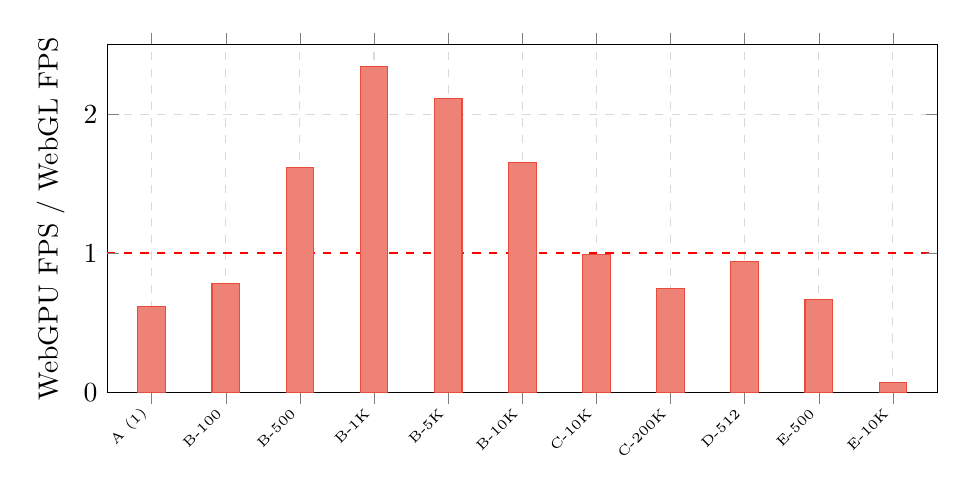
\begin{tikzpicture}
\begin{axis}[
    ybar,
    width=\columnwidth,
    height=6cm,
    bar width=10pt,
    ylabel={WebGPU FPS / WebGL FPS},
    symbolic x coords={A (1), B-100, B-500, B-1K, B-5K, B-10K, C-10K, C-200K, D-512, E-500, E-10K},
    xtick=data,
    x tick label style={font=\tiny, rotate=45, anchor=east},
    ymin=0, ymax=2.5,
    grid=major,
    grid style={dashed, gray!30},
    enlarge x limits=0.06,
    extra y ticks={1.0},
    extra y tick labels={},
    extra y tick style={grid=major, grid style={red, thick}},
]
\addplot[fill=webgpured!70, draw=webgpured] coordinates {
    (A (1), 0.618)
    (B-100, 0.784)
    (B-500, 1.618)
    (B-1K, 2.340)
    (B-5K, 2.113)
    (B-10K, 1.654)
    (C-10K, 0.990)
    (C-200K, 0.745)
    (D-512, 0.940)
    (E-500, 0.671)
    (E-10K, 0.074)
};
\end{axis}
\end{tikzpicture}
\caption{Cross-scenario FPS ratio (WebGPU/WebGL). Values above the red parity line (1.0) indicate WebGPU advantage; below indicates WebGL advantage. WebGPU excels only in instanced rendering (Scenario B, 500--10K) and is dramatically worse for state-change workloads (Scenario E).}
\label{fig:summary_radar}
\end{figure}

%----------------------------------------------------------------------
\section{Discussion}
\label{sec:discussion}

\subsection{When WebGPU Excels}

Our results identify two primary conditions under which WebGPU provides clear advantages:

\textbf{1) Instanced rendering at scale (Scenario B)}: When the number of rendered instances exceeds approximately 200, WebGPU's pre-compiled pipeline and efficient instance buffer management yield significantly higher throughput (up to 2.34$\times$ FPS) with dramatically better tail latency (P95 below 7.11~ms vs. WebGL's 53.88~ms). This advantage makes WebGPU compelling for applications rendering large 3D scenes, such as architectural visualization, terrain rendering, and particle-heavy effects using instanced geometry.

\textbf{2) GPU-side data-parallel computation (Scenario C)}: WebGPU's native compute shaders entirely offload particle physics to the GPU, keeping CPU overhead constant at $\sim$0.5~ms regardless of particle count. This frees the main thread for other tasks (UI updates, network requests, application logic). For applications requiring large-scale simulations (fluid dynamics, molecular visualization, machine learning inference in the browser), this represents a qualitative, not merely quantitative, advantage.

\subsection{When WebGL Remains Competitive}

\textbf{1) Low-complexity rendering (Scenario A)}: For simple scenes with few draw calls, WebGL's lower per-frame overhead and mature driver optimization yield 1.62$\times$ superior FPS. Applications such as product configurators or basic data visualizations with limited geometry may not benefit from WebGPU.

\textbf{2) State-change-heavy rendering (Scenario E)}: WebGL significantly outperforms WebGPU when each object requires unique pipeline state (unique uniforms, separate draw calls). At 10{,}000 objects, WebGL achieves 13.6$\times$ higher FPS with frame time stability ($\sigma_{\text{FPS}} = 1.51$) versus WebGPU's extreme instability ($\sigma_{\text{FPS}} = 0.27$ at convergence, but prior counts show $\sigma = 83.68$). This pattern is common in applications that cannot use instancing---for example, scenes with heterogeneous objects requiring different materials, blend states, or shader programs.

\textbf{3) GPU-bound compute workloads (Scenario D)}: When the workload is purely GPU-compute-bound, both APIs achieve similar throughput (within 11\%), as the GPU is the bottleneck rather than the API. WebGL's render-to-texture GPGPU approach, while less elegant, performs comparably.

\subsection{Initialization Overhead}

WebGPU's high initialization latency (Table~\ref{tab:init_time}) has practical implications for application startup time and dynamic resource creation. The most extreme case---Scenario~E at 10K objects with 3.25~seconds of initialization---would cause a noticeable delay before the first frame. Applications that frequently create or modify pipelines, bind groups, or shader modules will incur repeated delays. Strategies to mitigate this include pipeline caching, lazy initialization, precompilation of commonly used shader modules, and amortizing bind group creation across frames. WebGPU implementations are also expected to improve initialization performance as browser engines mature.

\subsection{Tail Latency Implications}

The P95 analysis reveals an important nuance not captured by mean FPS alone. In Scenario~B, WebGL's mean FPS of 162.69 (at 1K instances) masks a P95 frame time of 53.88~ms---well above the 16.67~ms budget for 60~Hz rendering. This means that while WebGL achieves acceptable \textit{average} performance, users will experience periodic stutter. WebGPU's P95 of 4.09~ms at the same count ensures consistently smooth animation, which is critical for VR/AR applications where frame drops cause motion sickness.

\subsection{State-Change Pattern Analysis}

The severe WebGPU degradation in Scenario~E warrants deeper analysis. In our WebGPU implementation, each object requires updating a distinct bind group to modify its model-view matrix and color uniform. This results in $N$ \texttt{setBindGroup} and $N$ \texttt{drawIndexed} calls per frame. The overhead likely stems from WebGPU's validation layer, which must verify bind group compatibility with the pipeline layout on every \texttt{setBindGroup} call. This is a known limitation of the current WebGPU specification and browser implementations.

Developers can mitigate this by employing dynamic uniform buffers with dynamic offsets (a single large buffer with per-object ranges), indirect rendering with compute-shader-driven scene management, or multi-draw indirect commands. Reducing the number of unique bind groups per frame is critical for WebGPU performance in heterogeneous scenes.

\subsection{Threats to Validity}

Several factors may influence the generalizability of our results:

\begin{itemize}
    \item \textbf{Browser and driver maturity}: WebGPU is a nascent standard with rapidly evolving browser implementations. Performance characteristics may change significantly across browser versions.
    \item \textbf{Headless rendering}: Benchmarks were run in headless Chromium, which may differ from windowed rendering in display composition overhead.
    \item \textbf{Single hardware configuration}: Results are specific to one GPU/driver combination. Different hardware (especially integrated vs.\ discrete GPUs, mobile vs.\ desktop) may show different scaling behavior.
    \item \textbf{Implementation choices}: The Scenario~E WebGPU implementation uses per-object bind groups, which represents a worst-case pattern. Optimized implementations using dynamic uniform buffers could reduce the performance gap.
\end{itemize}

%----------------------------------------------------------------------
\section{Conclusion and Future Work}
\label{sec:conclusion}

This paper presents the first comprehensive, automated benchmarking comparison between WebGL~2.0 and WebGPU across five distinct rendering and compute scenarios. Our key findings are:

\begin{enumerate}
    \item WebGPU achieves up to \textbf{2.34$\times$} higher FPS for instanced rendering workloads with \textbf{7.6$\times$ lower tail latency} (P95), making it the superior choice for geometry-intensive applications requiring smooth frame delivery.
    \item WebGPU's compute shaders reduce CPU overhead by up to \textbf{89.6\%} compared to WebGL's CPU-based particle simulation, enabling larger data-parallel workloads without blocking the main thread.
    \item WebGL remains \textbf{13.6$\times$} faster for state-change-heavy rendering patterns, where each object requires individual uniform updates and draw calls.
    \item WebGPU incurs \textbf{17--383$\times$} higher initialization overhead, with worst-case startup exceeding 3 seconds for complex bind group configurations.
    \item For GPU-bound compute workloads, both APIs achieve comparable steady-state throughput (within 11\%), confirming that the GPU, not the API, is the bottleneck.
\end{enumerate}

These results provide empirically grounded, scenario-specific guidance for web developers. We recommend WebGPU for new applications with instanced rendering, GPU compute requirements, or large-scale simulations. Applications with many heterogeneous objects requiring individual draw calls should carefully evaluate the state-change overhead before migrating from WebGL.

Future work includes: (1) extending benchmarks to mobile browser platforms (Chrome Android, Safari WebKit), (2) evaluating optimized WebGPU patterns (dynamic uniform buffers, indirect drawing, multi-draw) for state-change-heavy workloads, (3) comparing multi-threaded command encoding strategies using Web Workers, (4) longitudinal tracking of performance across browser releases as WebGPU matures, and (5) incorporating additional benchmark scenarios such as shadow mapping, deferred rendering, post-processing pipelines, and texture streaming.

\section*{Data Availability}

The benchmarking framework, complete source code, and all raw experimental data (JSON and CSV) are open-source and available in the accompanying repository for full reproducibility.

\section*{Acknowledgments}

The authors thank the W3C GPU for the Web Community Group for the WebGPU specification and the Chromium team for their implementation efforts.

%----------------------------------------------------------------------
% References
%----------------------------------------------------------------------
\bibliographystyle{IEEEtran}
\bibliography{references}

\balance

\end{document}
